\univlogo

{\Huge April 23}\vspace{5mm}

\section*{Face recognition example in chapter 4}

\subsection*{Task}

Greyscale image number: 624

Resolution: $120 \times 128$

Greyscale intensity: 8 bit (0:black, 255:white)

\begin{LARGE}Learning\end{LARGE} the direction in which the person is facing (left, right, straight ahead, or upward)

\subsection*{Input encoding}

The ANN input is to be some representation of the image, one key design choice is how to encode this image. For example, we could preprocess the image to extract edges, regions of uniform intensity, or other local image features, then input these features to the network.

In this case, we choose to encode the image as a fixed set of $30 \times 32$ pixel intensity values, with \textbf{one network input per pixel}. The pixel intensity values ranging from 0 to 255 were linearly scaled to range from 0 to 1 so that network inputs would have values in the same interval as the hidden unit and output unit activations.

The $30 \times 32$ pixel image is a coarse resolution of the original $120 \times 128$ captured image, with each coarse pixel intensity calculated as the mean of the corresponding high-resolution pixel intensities. However in ALVINN, each coarse resolution pixel intensity is obtained by selecting the intensity of a single pixel at random from the appropriate region within the high-resolution image, rather than taking the mean of all pixel intensities within this region. The motivation for this in ALVINN is that it significantly reduces the computation required to produce the coarse-resolution image from the available high-resolution image. This efficiency is especially important when the network must be used to process many images per second while autonumously driving the vehicle.

\subsection*{Output encoding}

Left, right, up, or straight? The ANN must output one of them.

We could encode this four-way classification using a single output unit, assigning outputs of 0.2, 0.4, 0.6, and 0.8 to encode these four possible values. However we use \textbf{four distinct output units}, each representing one of the four possible face directions, with the highest-valued putput taken as the network prediction.(often called a 1-of-n output encoding)

Two reasons for choosing the 1-of-n output encoding:

- It provides \textbf{more degrees of freedom} to the network for representing the target function.

- In the 1-of-n encoding \textbf{the differece between the highest-valued output and the second-highest can be used as a measure of the confidence} in the network prediction (ambiguous classifications may result in near or exact ties).

Instead of using $<1,0,0,0>$ to encode a left-looking face and $<0,1,0,0>$ to encode a straight-looking face, we use values of 0.9 and 0.1 because \textbf{sigmoid units cannot produce these outpout valuesgiven finite weights}. If we attempt to train the network to fit target values of exactly 0 and 1, gradient descent will force the weights to grow without bound. On the other hand, values of 0.1 and 0.9 are achievable using a sigmoid unit with finite weights.

\subsection*{Network graph structure}

The most common network structure is a layered network with feedforward connections from every unit in one layer to every unit in the next which we choose to use in the current design, using two layers of sigmoid units (one hidden layer and one output layer).

\subsection*{Other learning algorithm parameters}

learning rate $\eta = 0.3$

momentum $\alpha = 0.3$

Lower values for both parameters produced roughly equivalent generalization accuracy but longer training times. If these values are set too high, training fails to converge to a network with acceptable error over the tarining set.

Full gradient descent was used.

Network weights in the output units were initialized to small random values. However, input unit weights were initialized to 0 to yield much more intelligible visualizations of learned weights, without any noticeable impact on generalization accuracy.

The number of training iterations was selected by partitioning the available data into a \textbf{training set} and a separate \textbf{validation set}.

\textbf{Gradient descent} was used to minimize the error over the training set.

The performance of the network was evaluated over the validation set after \textbf{every 50 gradient descent steps}.

\begin{figure}[H]
    \centering
    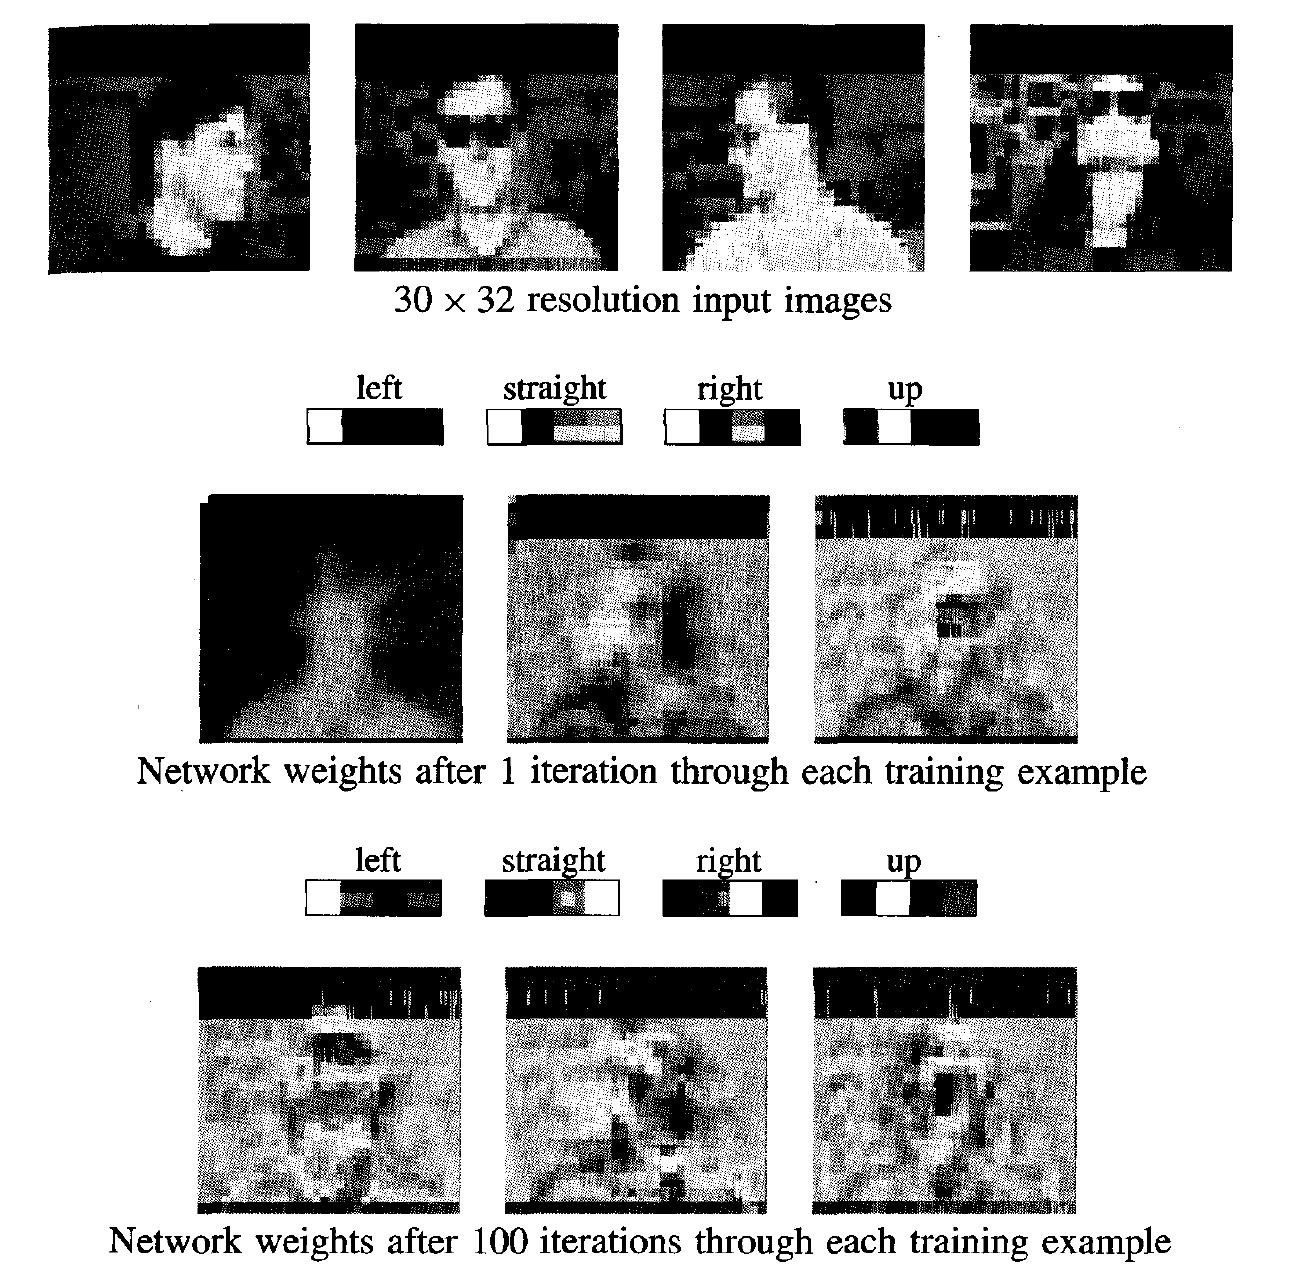
\includegraphics[width=0.6\textwidth]{./2023April/faceRecog.png}
    \caption{Process of training}
    \label{faceRecognition}
\end{figure}

\begin{figure}[H]
    \centering
    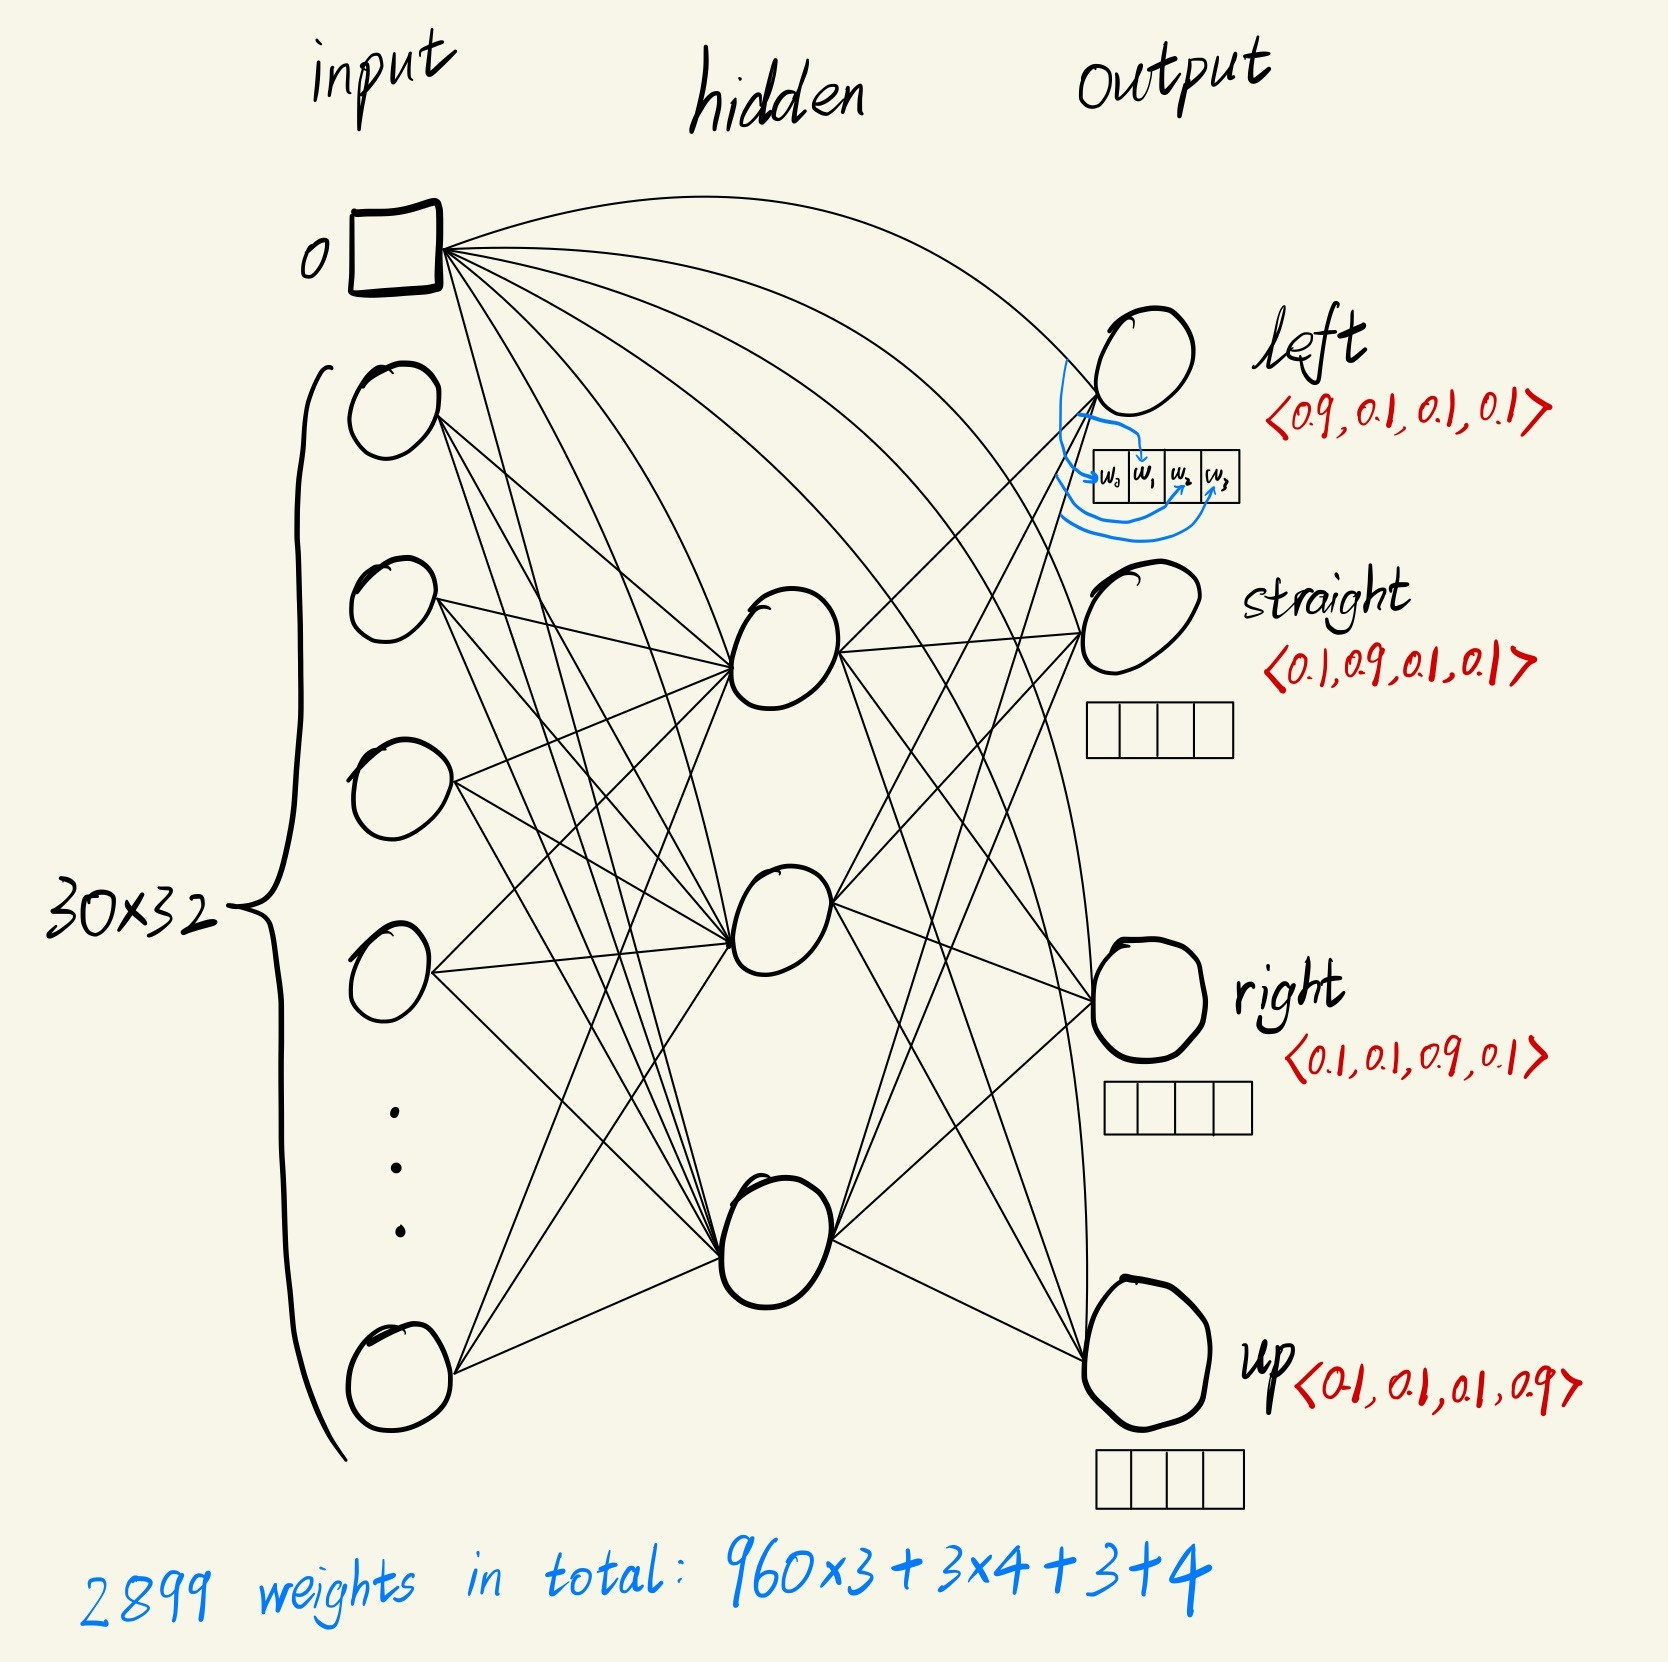
\includegraphics[width=0.55\textwidth]{./2023April/faceRecogLayer.png}
    \caption{Layers}
    \label{faceRecognitionLayers}
\end{figure}

As is shown above, the four squares within each rectangle indicate the four weights associated with this output unit--the weight $w_0$, which determines the unit \textbf{threshhold}(on the left), followed by the three weights connecting the three hidden units to this output.

The \textbf{brightness} of the square indicates the weight value, with \textbf{bright white} indicating a large positive weight, \textbf{dark black} indicating a large negative weight, and intermediate shades of \textbf{grey} indicating intermediate weight values.



